\documentclass[tikz,border=10pt]{standalone}
\usepackage{amsmath}
\definecolor{aksen}{HTML}{F7B538}
\definecolor{latar}{HTML}{171D2B}
\pagecolor{latar}
\begin{document}
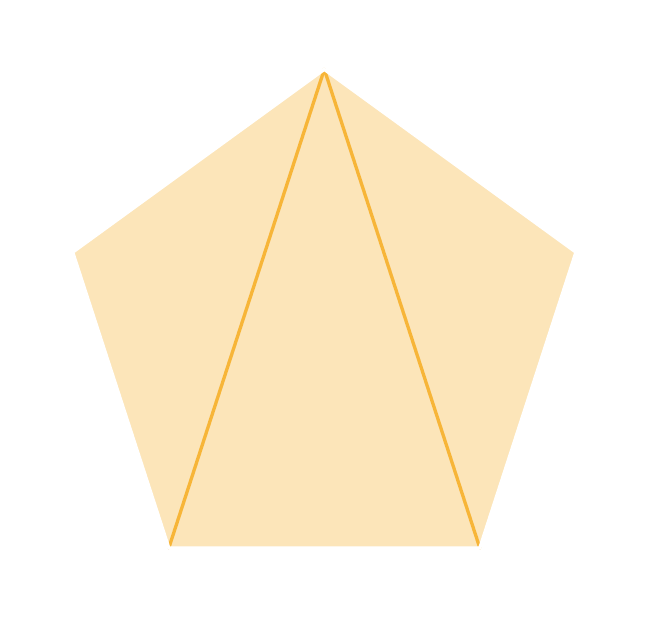
\begin{tikzpicture}[
  scale=2.4,
  line cap=round,
  every node/.style={text=white, font=\large},
  segitiga/.style={fill=aksen!35, draw=white, thick},
  garisbagi/.style={draw=aksen, very thick}
]
  % Segi lima beraturan dari koordinat polar (pusat di O, radius 1.4)
  \coordinate (A) at (90:1.4);
  \coordinate (B) at (18:1.4);
  \coordinate (C) at (-54:1.4);
  \coordinate (D) at (-126:1.4);
  \coordinate (E) at (162:1.4);
  % Tiga segitiga hasil pembagian dari titik A
  \fill[segitiga] (A) -- (B) -- (C) -- cycle;
  \fill[segitiga] (A) -- (C) -- (D) -- cycle;
  \fill[segitiga] (A) -- (D) -- (E) -- cycle;
  % Garis bagi
  \draw[garisbagi] (A) -- (C);
  \draw[garisbagi] (A) -- (D);
  % Keliling bangun
  \draw[white, very thick] (A) -- (B) -- (C) -- (D) -- (E) -- cycle;
  % Label titik
  \node[above] at (A) {$A$};
  \node[right] at (B) {$B$};
  \node[below right] at (C) {$C$};
  \node[below left] at (D) {$D$};
  \node[left] at (E) {$E$};
\end{tikzpicture}
\end{document}
